
\section*{Time Domain Full Waveform Inversion}
\subsection{Seismic Acquisition}

%% %%%%%%%%%%%%%%%%%%%%%%%%%%%%%%%%%%%%%%%%%%%%%%%%%%%%%% 2 %%%%%%%%%%%%%%%%%%%%%%%%%%%%%%%%%%%%%%%%%%%%%%%%%%%%%%%%%%%%%%%%%%%%%%%%%%%%%%%%%b%%%%%%%%%%%%%%%%%%%
\begin{frame}{Seismic Acquisition}


  \begin{figure}
    \def\svgwidth{1.05\linewidth}
    \input{images/intro_1.pdf_tex}
  \end{figure}

\end{frame}

\begin{frame}[noframenumbering]{Seismic Acquisition}


  \begin{figure}
    \def\svgwidth{1.05\linewidth}
    \input{images/intro_2.pdf_tex}
  \end{figure}

\end{frame}
%%%%%%%%%%%%%%%%%%%%%%%%%%%%%%%%%%%%%%%%%%%%%%%%%%%%%% 2 %%%%%%%%%%%%%%%%%%%%%%%%%%%%%%%%%%%%%%%%%%%%%%%%%%%%%%%%%%%%%%%%%%%%%%%%%%%%%%%%%%%%%%%%%%%%%%%%%%%%%


%%%%%%%%%%%%%%%%%%%%%%%%%%%%%%%%%%%%%%%%%%%%%%%%%%%%%% 3 %%%%%%%%%%%%%%%%%%%%%%%%%%%%%%%%%%%%%%%%%%%%%%%%%%%%%%%%%%%%%%%%%%%%%%%%%%%%%%%%%%%%%%%%%%%%%%%%%%%%%
\newcommand\hideit[1]{%
  \only<0| handout:1>{\mbox{}}%
  \invisible<0| handout:1>{#1}}


\subsection{FWI Workflow}

\begin{frame}{FWI Workflow}
  \begin{columns}
    \column{\dimexpr\paperwidth-10pt}
    \begin{figure}
      \def\svgwidth{1.0\linewidth}
      \input{images/data.pdf_tex}
    \end{figure}
  \end{columns}
  \vspace{4.5cm}
~
\end{frame}

\begin{frame}[noframenumbering]{FWI Workflow}
  \begin{columns}
    \column{\dimexpr\paperwidth-10pt}
    \begin{figure}
      \def\svgwidth{1.0\linewidth}
      \input{images/data_2.pdf_tex}
    \end{figure}
  \end{columns}
  \vspace{1cm}
  \uncover<2->{
    Cost function to minimize :
    \begin{equation}
      \CF(m) = \frac{1}{2}||\textcolor{blue}{d_{obs}}-\textcolor{red}{\mathcal{F}(m)}||^2dt
    \end{equation}
 \begin{itemize}
   \item $\mathcal{F}(m)$ is the restriction on the receivers of the simulated waves in the media $m$. (With $m = \velocity, \density, \bulkmodulus$...)
   \item FWI iterates until $\CF(m) \longrightarrow 0$
 \end{itemize}
  }
\end{frame}

\begin{frame}{FWI Workflow}
\begin{figure}
  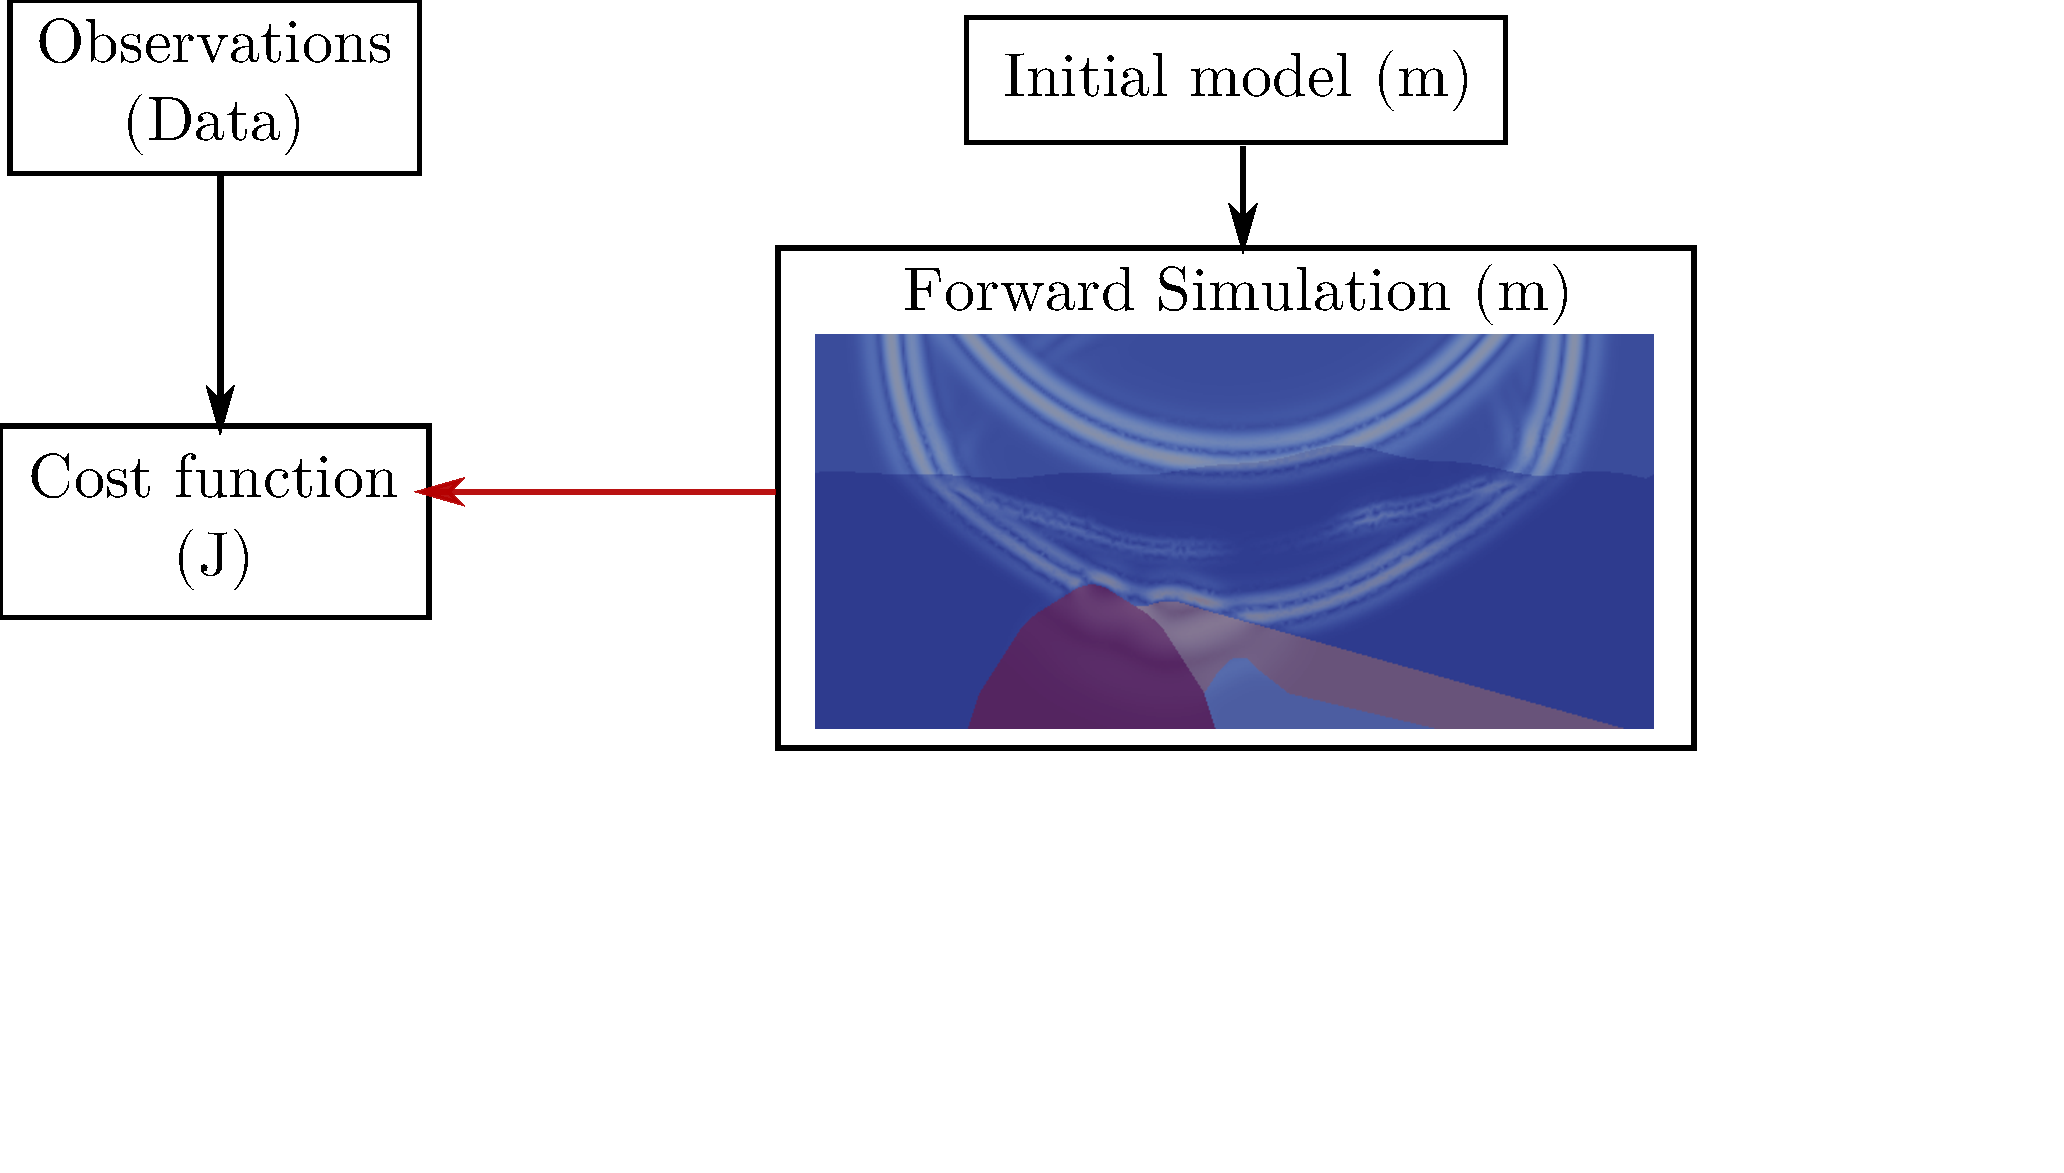
\includegraphics[scale=0.31]{fwi_test1.pdf}
\end{figure}
\end{frame}

\begin{frame}[noframenumbering]{FWI Workflow}
\begin{figure}
  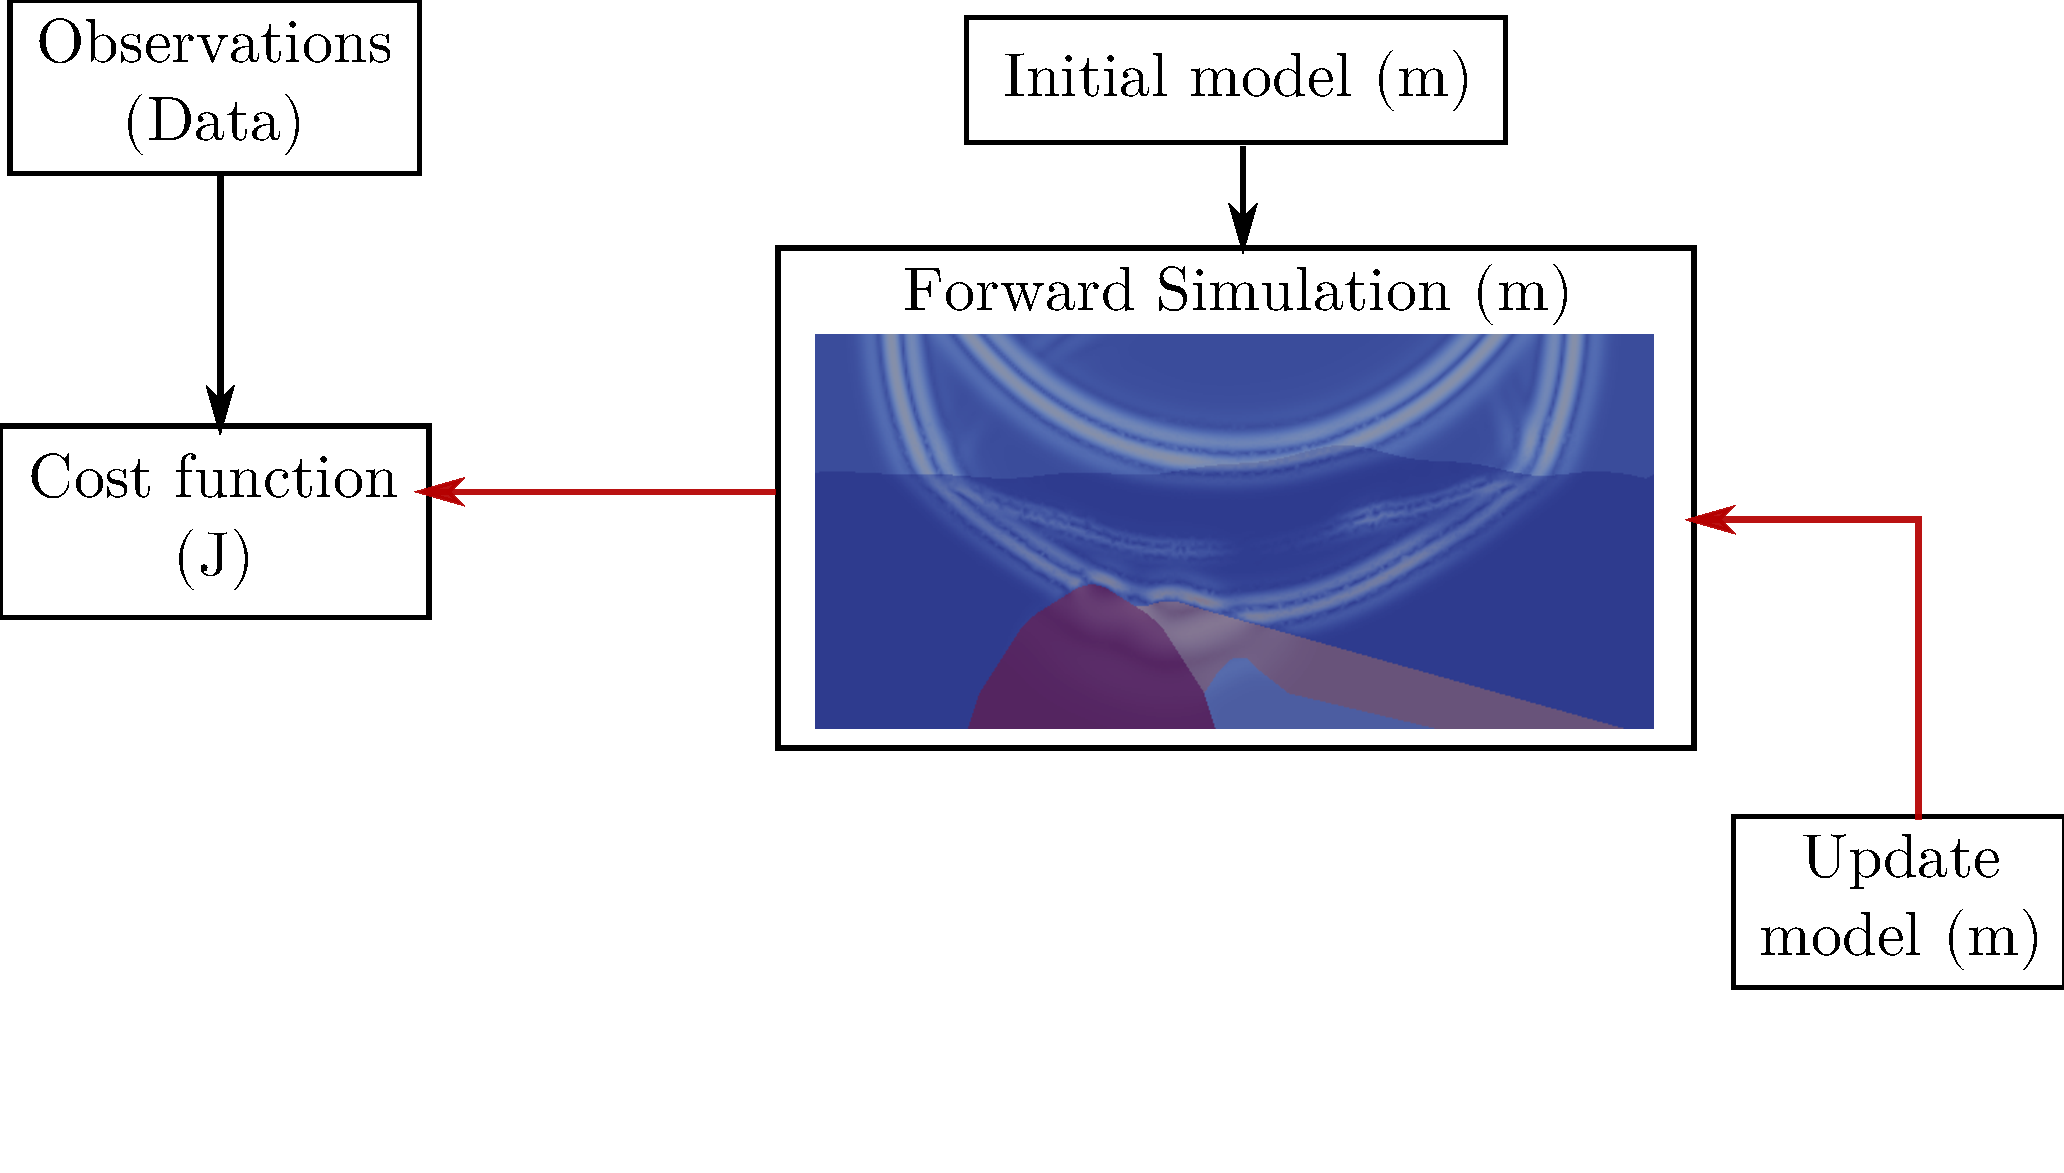
\includegraphics[scale=0.31]{fwi_test2.pdf}
\end{figure}
\end{frame}


\begin{frame}[noframenumbering]{FWI Workflow}
\begin{figure}
  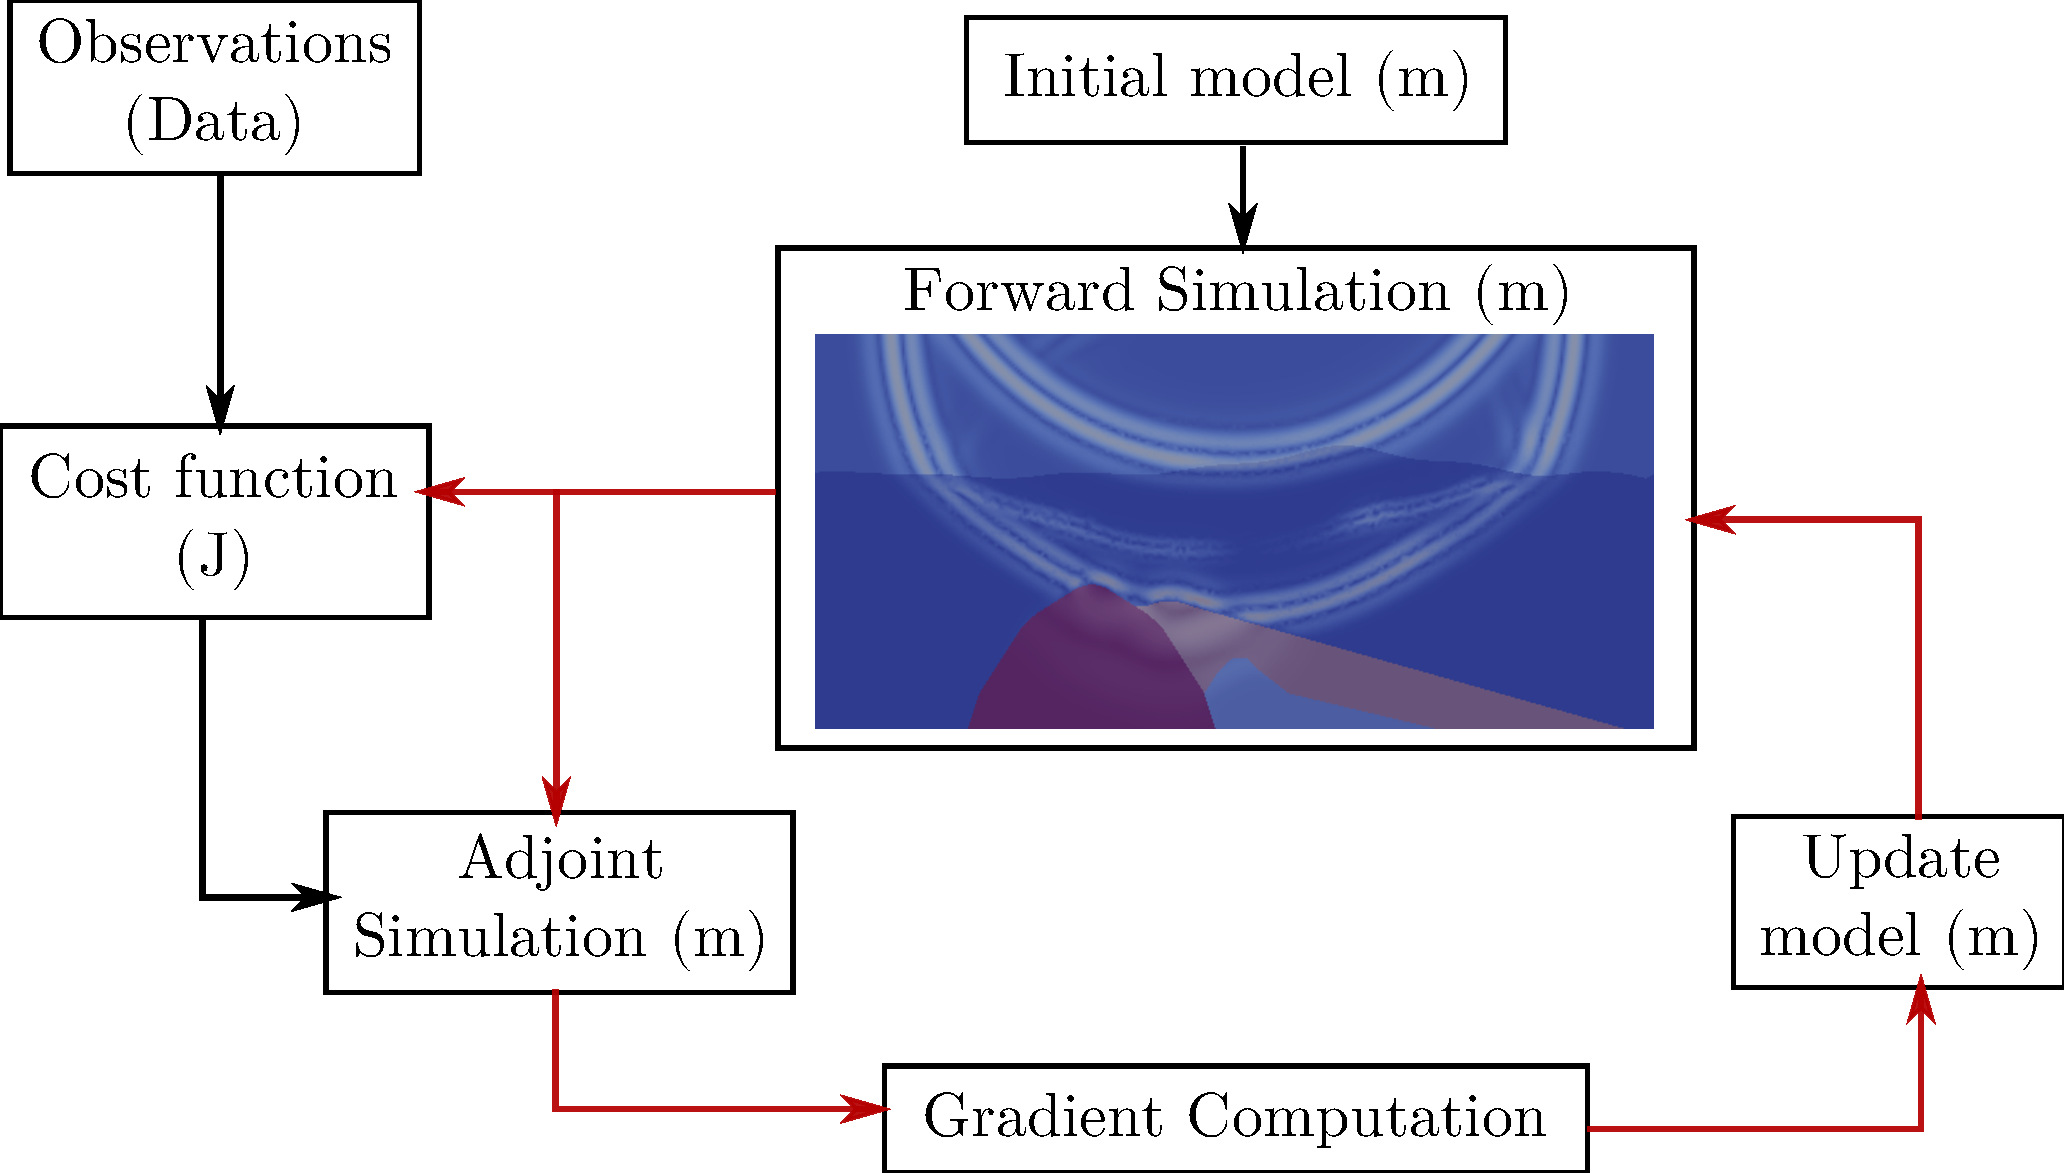
\includegraphics[scale=0.31]{fwi_test.pdf}
\end{figure}
\end{frame}

\begin{frame}[noframenumbering]{FWI Workflow}
\begin{figure}
  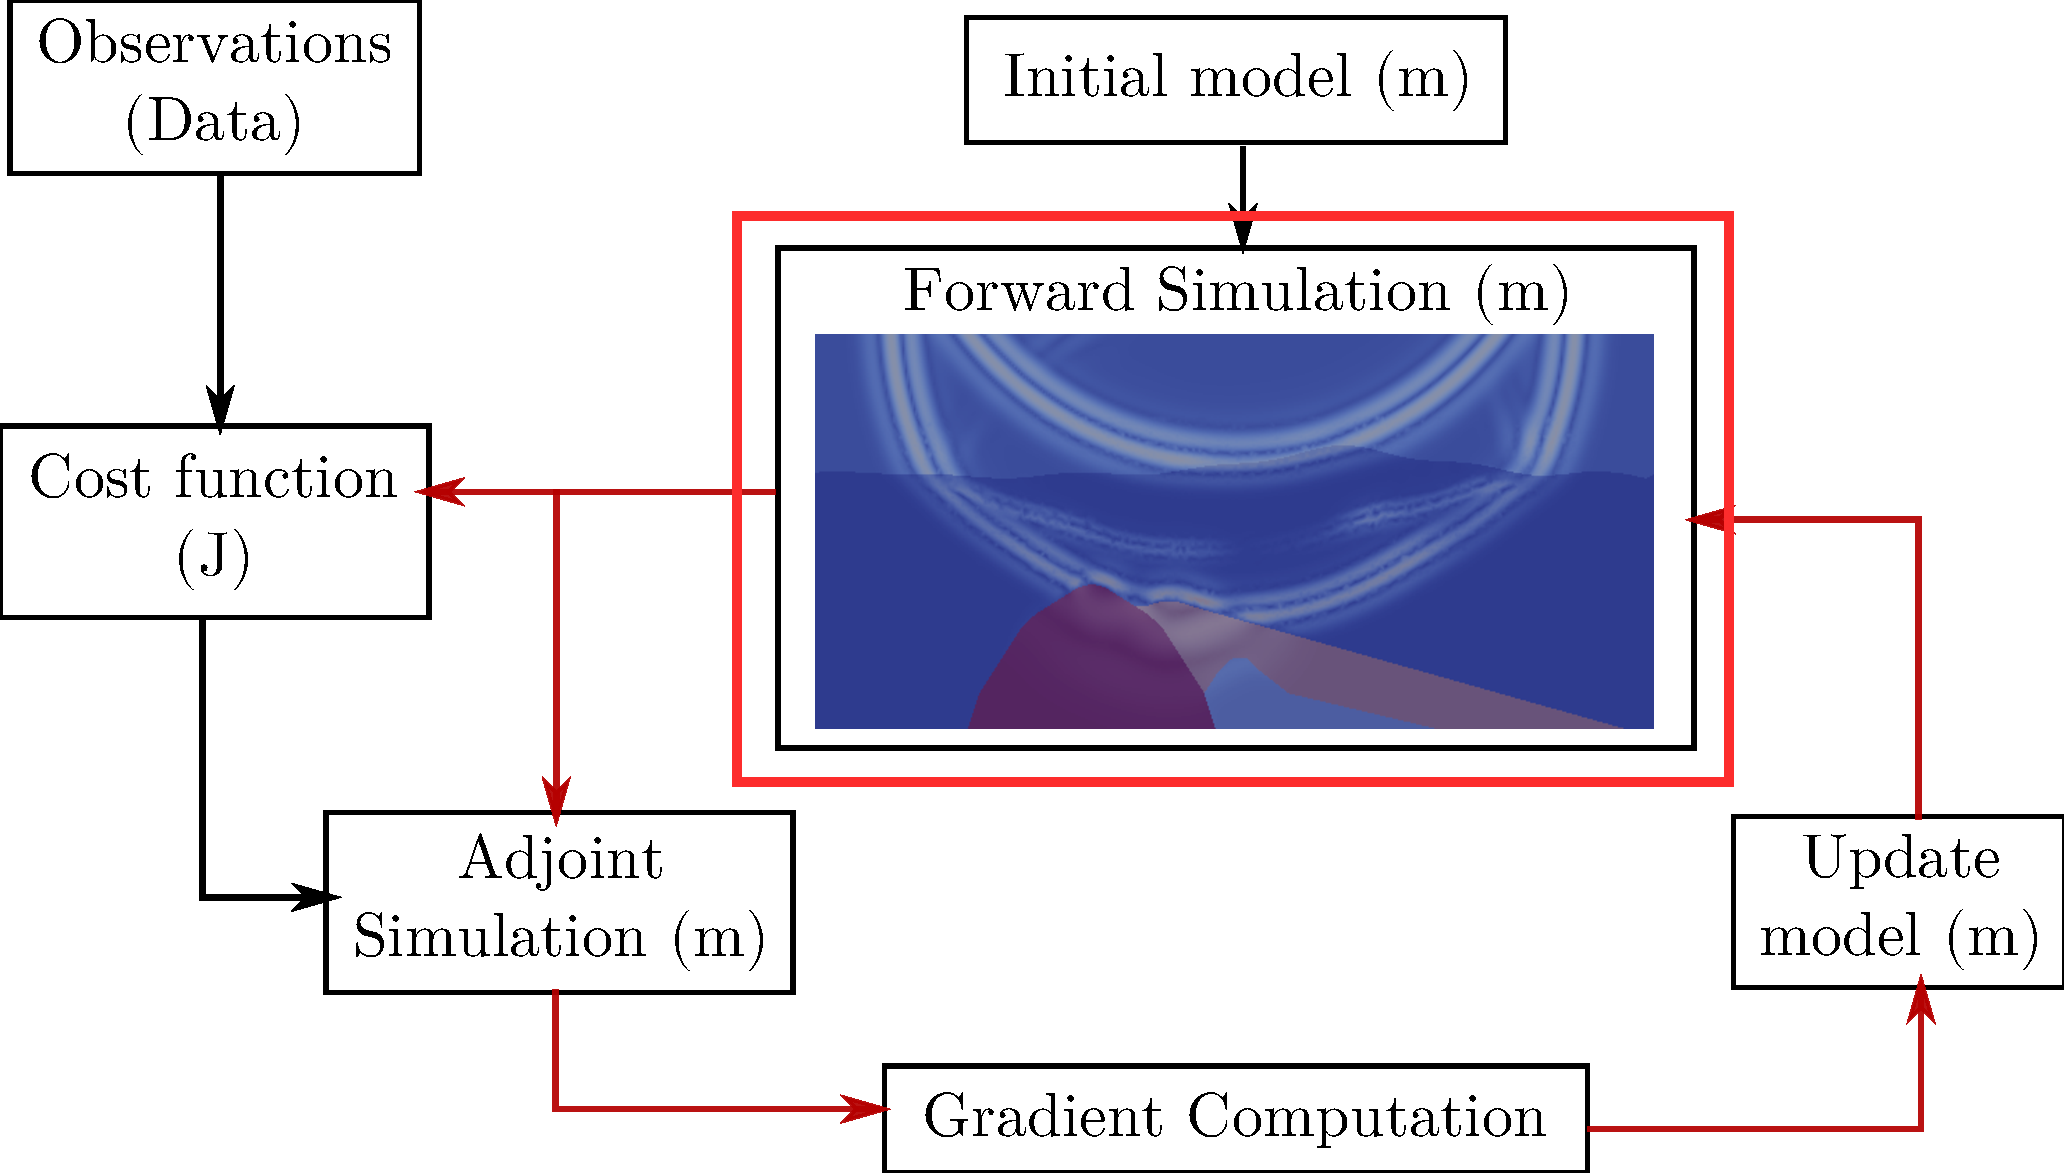
\includegraphics[scale=0.31]{fwi_test3.pdf}
\end{figure}
\end{frame}



\subsection{Forward Discretization}
\begin{frame}{Continuous Forward Model}

  First order acoustic wave equation
  \begin{multicols}{2}
  \begin{empheq}[left=\empheqlbrace]{align}
    & \frac{1}{\density \velocity^2}\frac{\partial \contP}{\partial t}+\nabla \cdot \contV=f_p \text{~~ on $\boldsymbol{\Omega}$}\\
    & \density\frac{\partial \contV}{\partial t}+\nabla\contP=f_v  \text{~~ on $\boldsymbol{\Omega}$}\\
    & \contP=0 \text{~~ on $\textcolor{red}{\boldsymbol{\Gamma_1}}$} \\
    & \frac{\partial \contP}{\partial t}+\velocity \nabla \contP \cdot \normal=0 \text{~~ on $\textcolor{blue}{\boldsymbol{\Gamma_2}}$}
  \end{empheq}

  \columnbreak

  \begin{center}
    \renewcommand\tikzscale{1.0}
    \begin{figure}[H]
    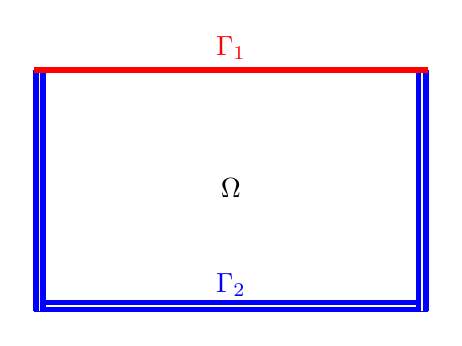
\begin{tikzpicture}[scale=\tikzscale]
\draw[color=blue,line width=2,double] (0,0) -- (5,0);
\draw[color=blue,line width=2,double] (0.07,-0.07) -- (0.07,3);
\draw[color=blue,line width=2,double] (4.93,-0.07) -- (4.93,3);
\draw[color=red,line width=2.1](-0.,3) -- (5,3);


\node[anchor=south, color=red]
at (2.5,3) {$\Gamma_1$};

\node[anchor=south, color=blue]
at (2.5,0) {$\Gamma_2$};

\node[color=black]
at (2.5,1.5) {$\Omega$};
\end{tikzpicture}

    \caption{Domain with Absorbing Boundary Conditions}
    \end{figure}
  \end{center}

  \end{multicols}
\end{frame}


\begin{frame}{Discrete Forward Model}

  \begin{multicols}{2}

    Space Discretization : Discontinuous Galerkin Elements
    \begin{itemize}
      \item Nodal (Lagrangian / Jacobian)
      \item Modal (Bernstein-Bézier)
    \end{itemize}
    \vspace{1cm}
    \uncover<3->{
    Time schemes :
    \begin{itemize}
      \item Runge Kutta 2/4
      \item Adams Bashforth 3
    \end{itemize}}

    \columnbreak

    \uncover<2->{
    Semi-discretized model :
    \begin{equation}
      \frac{\partial}{\partial t}\discreteU(t) = A \discreteU(t) + \discreteF(t)
    \end{equation}

    with :

    \begin{equation}
      \discreteU(t)=\vectll{(}{\discreteP(t)}{\discreteV(t)}{)}
    \end{equation}}

    \uncover<3->{
    \begin{figure}
      \noindent
       \begin{tikzpicture}[scale=0.8]
      \draw[color=black,line width=2.1](0.0,0.0) -- (5,0.0);
      %\draw[color=blue, line width=10] (0,-0.02) node {$\bullet$} ;
      %\draw[color=blue, line width=10] (5,-0.02) node {$\bullet$} ;
     % \draw node[color=blue,fill,circle,minimum size=0.01](1,1) {};
      \node[anchor=south east, color=black]
      at (0,0) {$0$};
      \node[anchor=south west, color=black]
      at (5,0) {$T$};
      
      \pgfmathsetmacro{\x}{0.0}
      \draw[color=black,line width=2.1](\x,0.1) -- (\x,-0.1);

      \pgfmathsetmacro{\x}{5.0}
      \draw[color=black,line width=2.1](\x,0.1) -- (\x,-0.1);

      \pgfmathsetmacro{\x}{0.5}
      \draw[color=black,line width=1.5](\x,0.1) -- (\x,-0.1);
      \draw[arrowStyle,color=blue]
      (\x-0.5,0) to[out=90,in=90,looseness=4.0]
      node[sloped,anchor=south]
      {}
      (\x,0.0);
      \draw[color=black,line width=1.5](\x,0.1) -- (\x,-0.1);


      
      \pgfmathsetmacro{\x}{1.0}
            \draw[arrowStyle,color=blue]
      (\x-0.5,0) to[out=90,in=90,looseness=4.0]
      node[sloped,anchor=south]
      {}
      (\x,0.0);
      \draw[color=black,line width=1.5](\x,0.1) -- (\x,-0.1);
      \pgfmathsetmacro{\x}{1.5}
            \draw[arrowStyle,color=blue]
      (\x-0.5,0) to[out=90,in=180,looseness=1.0]
      node[sloped,anchor=south]
      {}
      (\x,0.55);

      
      \draw[color=black,line width=1.5](\x,0.1) -- (\x,-0.1);
      \pgfmathsetmacro{\x}{2.0}
      \draw[color=black,line width=1.5](\x,0.1) -- (\x,-0.1);
      \pgfmathsetmacro{\x}{2.5}
      \draw[color=black,line width=1.5](\x,0.1) -- (\x,-0.1);
      \pgfmathsetmacro{\x}{3.0}
      \draw[color=black,line width=1.5](\x,0.1) -- (\x,-0.1);
      \pgfmathsetmacro{\x}{3.5}
      \draw[color=black,line width=1.5](\x,0.1) -- (\x,-0.1);
      \pgfmathsetmacro{\x}{4.0}
      \draw[color=black,line width=1.5](\x,0.1) -- (\x,-0.1);
      \pgfmathsetmacro{\x}{4.5}
      \draw[color=black,line width=1.5](\x,0.1) -- (\x,-0.1);
    \end{tikzpicture}

      Forward time steps
    \end{figure}}

  \end{multicols}

\end{frame}


\begin{frame}{Discrete Forward Model}{Discontinuous Galerkin Method}
  Asset of Discontinuous Galerkin Methods : \\

  \begin{itemize}
  \item Unstructured grid (enable to match the topography and media irregularities)
  \item Robust to physical discontinuities
  \item hp-adaptivity
  \item Massively parallel performance properties
  \end{itemize}

  \begin{figure}[H]
    \subfigure[h-adaptivity]{
      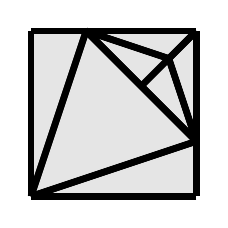
\begin{tikzpicture}[scale=0.7]%[line cap=round,line join=round,>=triangle 45,x=1.0cm,y=1.0cm]
      %% \draw[->,color=black] (-1.05,0) -- (9.66,0);
      %% \foreach \x in {-1,-0.5,0.5,1,1.5,2,2.5,3,3.5,4,4.5,5,5.5,6,6.5,7,7.5,8,8.5,9,9.5}
      %% \draw[shift={(\x,0)},color=black] (0pt,2pt) -- (0pt,-2pt) node[below] {\footnotesize $\x$};
      %% \draw[->,color=black] (0,-0.43) -- (0,5.53);
      %% \foreach \y in {,0.5,1,1.5,2,2.5,3,3.5,4,4.5,5,5.5}
      %% \draw[shift={(0,\y)},color=black] (2pt,0pt) -- (-2pt,0pt) node[left] {\footnotesize $\y$};
      %% \draw[color=black] (0pt,-10pt) node[right] {\footnotesize $0$};
      %% \clip(-1.05,-0.43) rectangle (9.66,5.53);
      \fill[line width=2.4pt,fill=black,fill opacity=0.1] (1,1) -- (4,2) -- (4,1) -- cycle;
      \fill[line width=2.4pt,fill=black,fill opacity=0.1] (1,1) -- (1,4) -- (2,4) -- cycle;
      \fill[line width=2.4pt,fill=black,fill opacity=0.1] (2,4) -- (4,2) -- (1,1) -- cycle;
      \fill[line width=2.4pt,fill=black,fill opacity=0.1] (2,4) -- (4,4) -- (4,2) -- cycle;
      \draw [line width=2.4pt] (1,1)-- (4,2);
      \draw [line width=2.4pt] (4,2)-- (4,1);
      \draw [line width=2.4pt] (4,1)-- (1,1);
      \draw [line width=2.4pt] (1,1)-- (1,4);
      \draw [line width=2.4pt] (1,4)-- (2,4);
      \draw [line width=2.4pt] (2,4)-- (1,1);
      \draw [line width=2.4pt] (2,4)-- (4,2);
      \draw [line width=2.4pt] (4,2)-- (1,1);
      \draw [line width=2.4pt] (1,1)-- (2,4);
      \draw [line width=2.4pt] (2,4)-- (4,4);
      \draw [line width=2.4pt] (4,4)-- (4,2);
      \draw [line width=2.4pt] (4,2)-- (2,4);
      \draw [line width=2.4pt] (2,4)-- (3.5,3.5);
      \draw [line width=2.4pt] (3,3)-- (4,4);
      \draw [line width=2.4pt] (4,4)-- (2,4);
      \draw [line width=2.4pt] (2,4)-- (3.5,3.5);
      \draw [line width=2.4pt] (3.5,3.5)-- (4,2);
      \draw [line width=2.4pt] (4,2)-- (2,4);
      \draw [line width=2.4pt] (4,2)-- (4,4);
      \draw [line width=2.4pt] (4,4)-- (3.5,3.5);
      \draw [line width=2.4pt] (3.5,3.5)-- (4,2);
  \end{tikzpicture}

}
    \hspace{1cm}
  \subfigure[p-adaptivity with \textcolor{black}{P1}, \textcolor{blue}{P2}, \textcolor{red}{P3} elements]{
      \definecolor{ccqqqq}{rgb}{0.8,0,0}
    \definecolor{qqqqff}{rgb}{0,0,1}
    \definecolor{cccccc}{rgb}{0.8,0.8,0.8}
    \begin{tikzpicture}[scale=0.7]
      %\draw[->,color=black] (0,0.62) -- (0,4.91);
      %\foreach \y in {0.6,0.8,1,1.2,1.4,1.6,1.8,2,2.2,2.4,2.6,2.8,3,3.2,3.4,3.6,3.8,4,4.2,4.4,4.6,4.8}
      %\draw[shift={(0,\y)},color=black] (2pt,0pt) -- (-2pt,0pt) node[left] {\footnotesize $\y$};
      %\clip(-0.64,0.62) rectangle (7.09,4.91);
      \fill[line width=1.6pt,color=cccccc,fill=cccccc,fill opacity=0.15] (1,1) -- (1,4) -- (4,4) -- (4,1) -- cycle;
      \fill[fill=black,fill opacity=0.1] (1,1) -- (2.5,2.5) -- (4,1) -- cycle;
      \fill[fill=black,fill opacity=0.1] (1,1) -- (2.5,2.5) -- (1,4) -- cycle;
      \fill[fill=black,fill opacity=0.1] (1,4) -- (4,4) -- (2.5,2.5) -- cycle;
      \fill[fill=black,fill opacity=0.1] (4,1) -- (2.5,2.5) -- (4,4) -- cycle;
      \draw [line width=2.8pt] (1,1)-- (1,4);
      \draw [line width=2.8pt] (1,4)-- (4,4);
      \draw [line width=2.8pt] (4,4)-- (4,1);
      \draw [line width=2.8pt] (4,1)-- (1,1);
      \draw [line width=2.8pt] (1,1)-- (2.5,2.5);
      \draw [line width=2.8pt] (2.5,2.5)-- (4,1);
      \draw [line width=2.8pt] (4,1)-- (1,1);
      \draw [line width=2.8pt] (1,1)-- (2.5,2.5);
      \draw [line width=2.8pt] (2.5,2.5)-- (1,4);
      \draw [line width=2.8pt] (1,4)-- (1,1);
      \draw [line width=2.8pt] (1,4)-- (4,4);
      \draw [line width=2.8pt] (4,4)-- (2.5,2.5);
      \draw [line width=2.8pt] (2.5,2.5)-- (1,4);
      \draw [line width=2.8pt] (4,1)-- (2.5,2.5);
      \draw [line width=2.8pt] (2.5,2.5)-- (4,4);
      \draw [line width=2.8pt] (4,4)-- (4,1);
      \begin{scriptsize}
        \fill [color=black] (1.07,3.76) circle (2.321pt);
        \fill [color=black] (1.08,1.24) circle (2.321pt);
        \fill [color=black] (2.3,2.5) circle (2.321pt);
        \fill [color=qqqqff] (2.51,2.3) circle (2.321pt);
        \fill [color=qqqqff] (2.72,2.5) circle (2.321pt);
        \fill [color=ccqqqq] (2.5,2.71) circle (2.321pt);
        \fill [color=qqqqff] (3.77,1.09) circle (2.321pt);
        \fill [color=qqqqff] (3.91,1.22) circle (2.321pt);
        \fill [color=ccqqqq] (3.73,3.87) circle (2.321pt);
        \fill [color=qqqqff] (3.89,3.75) circle (2.321pt);
        \fill [color=qqqqff] (1.24,1.11) circle (2.321pt);
        \fill [color=qqqqff] (1.87,1.7) circle (2.321pt);
        \fill [color=qqqqff] (3.14,1.69) circle (2.321pt);
        \fill [color=qqqqff] (2.51,1.1) circle (2.321pt);
        \fill [color=qqqqff] (3.31,1.86) circle (2.321pt);
        \fill [color=qqqqff] (3.9,2.48) circle (2.321pt);
        \fill [color=qqqqff] (3.31,3.13) circle (2.321pt);
        \fill [color=ccqqqq] (1.23,3.9) circle (2.321pt);
        \fill [color=ccqqqq] (2.08,3.87) circle (2.321pt);
        \fill [color=ccqqqq] (2.97,3.86) circle (2.321pt);
        \fill [color=ccqqqq] (1.63,3.56) circle (2.321pt);
        \fill [color=ccqqqq] (2.15,3.06) circle (2.321pt);
        \fill [color=ccqqqq] (3.36,3.54) circle (2.321pt);
        \fill [color=ccqqqq] (2.83,3.05) circle (2.321pt);
        \fill [color=ccqqqq] (2.49,3.55) circle (2.321pt);
      \end{scriptsize}
  \end{tikzpicture}

  }
\end{figure}
\end{frame}
